\chapter{KBBQ: A reference-free method for base quality score recalibration}
\label{ch:kbbq}
\section{Introduction}

Next generation sequencing has a plethora of applications in biology. %TODO: give some examples
While the technology is widely applied, the sequencing process is inherently erroneous and errors are common in sequencing data, with base substitution error rate estimates ranging between $.1$ and $1\%$, depending on the sequencing technology used \parencite{fox_accuracy_2014}.
To help mitigate this, DNA molecules are usually copied and sequenced multiple times to ensure the sequence is correct, since multiple independent measurements are unlikely to all contain the same error at the same position. While this works well in general, it can be costly and additional sample manipulation can damage samples and insert mutations, further increasing the amount of technical error in the data \parencite{schirmer_insight_2015, ma_analysis_2019}.

\subsection{Quality Scores}

In addition to increased sequencing depth, quality scores are an important part of sequencing data that helps identify erroneous sequences. Sequencing data is usually presented along with quality scores in the Phred scale \parencite{ewing_base-calling_1998, ewing_base-calling_1998-1}.
These quality scores measure the confidence the instrument has in its determination that any particular base in the sequence is correct.
Specifically, the quality score is equal to $-10\log_{10}P(e)$ \parencite{ewing_base-calling_1998} \parencite{ewing_base-calling_1998-1}, where $P(e)$ is the probability the base is an error.
For example, a base with a quality score of 40 has a .0001 probability of being incorrect while a base with a quality score of 10 has probability .1 of being incorrect. Generally, bases with scores lower than 10 are considered bad quality and bases with scores 30 and above are considered to be good quality. However, the score allows finer resolution than "good" and "bad", and is therefore more nuanced.

%new paragraph - importance
The usefulness of quantitative scores over categorical can be illustrated by considering how variant calling algorithms utilize quality scores.
Variant calling is a task to identify genetic variation in a sample from sequencing data.
Variant calling models use quality scores to differentially weight the observed data. Generally, these models attempt to find the sample genotype most consistent with the observed data and recognize that low quality bases provide less reliable evidence for one genotype over another. The BCFTools multiallelic caller \parencite{li_sequence_2009}, GATK's HaplotypeCaller \parencite{poplin_scaling_2018}, and FreeBayes \parencite{garrison_haplotype-based_2012}---three of the most popular variant callers---all take quality score into consideration when calling variants.
Since the quality score is an exactly defined probability, it is straightforward to integrate these scores into a model.

%new paragraph - binning
If so desired, quantitative scores can be collapsed into coarser categories, such as "good" and "bad". This is sometimes done as a heuristic; \textit{ie.} scores less than 10 are untrustworthy and filtered out of a dataset and other scores are trusted and retained.
The practice of binning quality scores together with neighboring scores is commonly performed to reduce file size \parencite{shibuya_better_2019, malysa_qvz_2015, yu_quality_2015, noauthor_reducing_2014}. 
However, it's important to note that this process cannot be simply reversed as information is lost when the scores are binned.

\subsection{Base Quality Score Recalibration}

% What is Base Quality Score Recalibration?
While base quality scores are important for identifying reliable data, base quality scores are often incorrect.
Base quality scores are exactly defined as a probability. They can be interpreted as a prediction giving the probability the reported base is an error. In general, probabilities are called \textit{calibrated} if the reported probability accurately predicts the frequency of an event.
Base quality scores in Illumina sequencing reads are not well-calibrated \parencite{callahan_dada2:_2016, ni_improvement_2016}. %(TODO: more cites)
A few alternative base calling models have been developed for Illumina machines that improve base call accuracy and quality score calibration; however, these are difficult to use because they require the raw output from the sequencing machine, which is unavailable to most users of sequencing as they are usually disposed of after a sequencing run due to the large cost associated with storing that data \parencite{kao_naivebayescall_2011, massingham_all_2012}. 


Since base quality scores are used to some degree by most variant calling methods, it is probable that poorly calibrated reads reduce the quality of resulting variant calls.
Similarly, the reduced amount of information in binned quality scores may also impact the quality of variant calls made using the data.
Poor calibration combined with poor resolution resulting from quality score binning may have an important impact on algorithms that rely on these scores to function, but the exact affect of these phenomena are unknown.

%actual BQSR
Though increased sequencing depth can help mitigate the impact of random sequencing errors, sequencing is affected by non-random biases.
For these types of errors, increasing sequencing depth counterintuitively \textit{increases} the effect of these errors, as they by definition occur preferentially at the same location. Thus, increased sequencing depth at that location adds more errors than are expected by chance, making those erroneous reads seem trustworthy. 
These biases can be due to the nature of the DNA sequence itself, with errors induced during library preparation or the sequencing reaction likely due to secondary structure \parencite{meacham_identification_2011, nakamura_sequence-specific_2011, schirmer_insight_2015, ma_analysis_2019}.
At the same time, the sequencing reaction is also non-randomly biased. Bases at the end of a read are much more likely to be erroneous than bases at the beginning of the read, and the identity of the base and adjacent bases also affect the error rate \parencite{fox_accuracy_2014, schirmer_illumina_2016}. 
Thus while random errors are troublesome, their impacts can be somewhat mitigated by more sequencing. Systematic errors cannot addressed in the same way, but they can be modeled and incorporated into quality scores.
%discuss non-random genomic locus vs. sequencing characteristics etc.    %non-random errors

% GATK BQSR occurs in 3 phases.
% Phase 1 - Count errors and covariates
Base quality score recalibration (BQSR) is the process of modeling errors in sequencing data and using the created model to update quality scores such that they reflect an accurate probability of error of any base.
GATK BQSR  is the most popular method for BQSR and is recommended before variant calling by the GATK best practices \parencite{auwera_fastq_2013}.
The model integrates many covariates of error such that the output quality score reflects an accurate, independent measure of the probability of error.
The algorithm takes reads aligned to a reference and a database of potentially variable sites in the genome as input.

The algorithm proceeds in 3 phases.
In the first phase, the algorithm compares each read to the aligned reference. Potentially variable sites are ignored and mismatches from the reference sequence and non-mismatches are counted. The numbers of matching and mismatching bases are categorized according to the model covariates, which are: read group, assigned quality score, sequencing cycle, and the base identity along with the identity of the previous base (the base context).
% Phase 2 - Train a hierarchical model.
In the second phase, a bayesian hierarchical model is trained with the count data. Using a normal distribution of the mean probability of error as a prior, the \textit{maximum a posteriori} (MAP) quality score of the read group is calculated assuming the errors are binomially distributed. That is,
\begin{align}
\hat{Q}_{rg} &= \operatorname{argmax}_{Q_{rg}} P(Q_{rg}|\operatorname{Errors}_{rg}) \\
&= \operatorname{argmax}_{Q_{rg}} P(\mathcal{B}(\operatorname{Errors}_{rg} | \operatorname{Observations}_{rg}, Q_{rg}) * P(\mathcal{N}(Q_{rg} | \bar{Q}))
\end{align}
This score is then used as the prior for calculating the \textit{maximum a posteriori} quality score for each assigned quality score in that read group, $\hat{Q}_{\operatorname{assigned\:quality\:score}}$, using a simular formula.
In turn, this score is used as the prior for calculating the \textit{maximum a posteriori} scores for the sequencing cycle and context covariates of bases with that score. The difference between the MAP estimate and the prior is used to calculate the final score, which is the sum of the MAP estimate of the assigned quality score and these two differences. That is,
\begin{align}
\Delta Q_{\operatorname{cycle}} &= \hat{Q}_{\operatorname{cycle}} - \hat{Q}_{\operatorname{assigned\:quality\:score}} \\
\Delta Q_{\operatorname{context}} &= \hat{Q}_{\operatorname{context}} - \hat{Q}_{\operatorname{assigned\:quality\:score}} \\
Q_{\operatorname{recalibrated}} &= \hat{Q}_{\operatorname{assigned\:quality\:score}} + \Delta Q_{\operatorname{cycle}} + \Delta Q_{\operatorname{context}}
\end{align}
In the third phase, the quality score of each read is adjusted based on the four covariates for each base in the read according to values calculated in the previous phase.

% How much does BQSR help?
BQSR improves quality score calibration in many cases, especially when there is moderate sequencing depth and the database of variable sites is nearly complete. %todo : cite
While BQSR is recommended in GATK's Best Practices, its affect on the resulting variant calls is not well-characterized, and there is ongoing debate about whether to continue recommending BQSR. \parencite{van_der_auwera_geraldine_2020, van_der_auwera_geraldine_2020_b}
However, \cite{ni_improvement_2016} find that improved quality score calibration aids detection of minor alleles in high coverage datasets by increasing sensitivity and reducing the number of false positive calls.
Thus, the need to perform BQSR and the performance of GATK's BQSR algorithm may vary from study to study.
One objective of this work is to help elucidate when GATK BQSR performs well and when it fails, and provide a method that works in situations that GATK BQSR struggles with.
As an example, the GATK developers recommend BQSR for use in cancer variant discovery \parencite{cibulskis_sensitive_2013}, but the tumor genome is likely much different from the human genome, and the database of variable sites will likely miss many truly variable sites due to the large mutation rate present in cancer genomes. Additionally, mismatches in reads misaligned due to chromosomal rearrangements may be mistakenly counted as evidence of sequencing error. The number of these errors required to significantly impact the performance of the algorithm is not clear.

\subsection{Alternative Approaches for BQSR}
% What is the problem with current methods for BQSR?
As illustrated above, the most problematic aspect of GATK BQSR occurs in the first phase of the algorithm: counting erroneous and non-erroneous bases. This is especially true when considering non-model organisms, where alignment errors may be common. Furthermore, in non-model organisms a database of variable sites is likely unavailable or largely incomplete. However, there are methods that attempt to overcome this deficiency. While there exist alternative approaches that implement different error models such as Lacer \parencite{chung_lacer:_2017}, the biggest problem for analyzing data without reliable reference information is the method of counting erroneous and non-erroneous bases.
% \item In a variant calling context, BQSR is probably most helpful in regions with low coverage, as the limited amount of data makes it difficult to differentiate between errors, heterozygous sites, and mutations.
 % or inconsistent coverage, as one may expect when sequencing a non-model organism; however, by definition that means no quality reference nor database of variable sites are available. Since these are required to perform GATK's BQSR, that means BQSR cannot be confidently completed.
% \item Find some estimates of differences between reference and samples sequenced; perhaps look at mouse
% \item This will be highly species-dependent and situation specific

% Alternative Approaches
Many alternative algorithms have been developed to avoid providing a database of variable sites. However, these approaches all still require a reference and alignment, and many require extra reagents and sequencing spike-ins that increase the cost of analysis and cannot be used to reanalyze existing sequencing data that hasn't been specially prepared.
% \item Lacer \parencite{chung_lacer:_2017} bins aligned bases based on depth and whether the base matches the reference, then uses singular value decomposition to infer the shift in quality score for each base.
ReQON \parencite{cabanski_reqon:_2012}, like GATK, considers bases that do not match the reference as errors but limits the number of acceptable errors at a position to minimize the effect of unknown variants. It then uses a logistic regression to recalibrate the quality scores.
SOAP2 \parencite{li_soap2:_2009} contains a model for consensus sequence construction that performs BQSR during construction. %It doesn't seem possible to get these recalibrated scores out??
The methods of \cite{zook_synthetic_2012} and \cite{ni_improvement_2016} use synthetic spike-ins of known composition and GATK's model \parencite{zook_synthetic_2012} or piecewise regression \parencite{ni_improvement_2016} to recalibrate quality scores. Since the sequence of the spike-in is known before hand, errors are easy to identify as there should be no biological variation in the spiked-in sample.
% \item While these approaches are useful alternatives to GATK, the comparisons presented here will only compare against GATK BQSR as none of the alternative approaches function without a reference and GATK BQSR is the most popular method.
Crucially, these methods require a reference and possibly other information to recalibrate reads that may not be available.

% kbbq
To effectively recalibrate base quality scores with as little auxiliary information as possible, I present \texttt{kbbq}, a software package to recalibrate quality scores of whole genome sequencing data without a reference or database of variable sites. The only required input is the set of reads to be recalibrated. Rather than excluding variation and comparing to the reference like GATK does, \texttt{kbbq} uses k-mer subsampling to find likely errors. Once the number of errors and nonerrors are counted and categorized according to their covariates, it uses the same model GATK uses to recalibrate the reads. I show how simulated false negatives and false positives affect GATK's ability to recalibrate reads and compare GATK calibration to \texttt{kbbq}.
\section{Methods}
	% \item Error correction algorithms
\texttt{kbbq} performs BQSR by adjusting how errors in the dataset are discovered.
Instead of looking at the reference, \texttt{kbbq} implements the error-correction algorithm described in \cite{song_lighter_2014} and uses the errors detected by that procedure to train and apply the standard GATK model. Note that the sequenced bases are not actually changed; the detected errors are used only to train the model. If there is evidence according to the model that the base is erroneous, its base quality will be decreased according to the strength of that evidence.

Briefly, the algorithm subsamples k-mers from the dataset. Since erroneous k-mers are expected to be unique, erroneous k-mers are less likely to be sampled than error-free k-mers. A binomial test is then conducted for every nucleotide in the dataset; if a sufficient number of k-mers contain the nucleotide, the base is likely not erroneous and called trusted. If \textit{k} of these trusted bases appear next to each other, that k-mer is stored as a trusted k-mer. Once the trusted k-mers have all been stored, each read is iterated through once again and any bases on the edge of an island of trusted k-mers are changed such that the change produces the maximal number of trusted k-mers in the read. These changes are marked as errors and used to train the model.
The model training and recalibration procedure are the same as those described above for GATK's BQSR method.

\subsection{Program Input and Parameters}

\texttt{kbbq} requires as input a set of reads in FASTQ \parencite{cock_sanger_2010} or BAM \parencite{li_sequence_2009} format. If the input data is FASTQ formatted and consists of multiple read groups, the read group each read belongs to should be annotated in the name of each read. Alternatively, if the user has an original data file and a data file that has already been corrected using an error correction program, the user may supply the corrected file with the \texttt{-\phantom{}-fixed} option to obtain errors from that correction rather than performing the error correction algorithm included in \texttt{kbbq}. The program's only required parameter is the approximate length of the sequenced region in base-pairs, and this information can be taken from the BAM header if it is present. It may be set with the \texttt{-\phantom{}-genomelen} option. If BAM input is provided, the \texttt{-\phantom{}-set-oq} and \texttt{-\phantom{}-use-oq} flags can be used to set the OQ flag on the read before recalibrating or to use the quality scores encoded in the OQ flag rather than the quality scores in the primary quality score field.

Optionally, the approximate sequencing coverage may also be provided with the \texttt{-\phantom{}-coverage} option. If it is not, it will be estimated by finding the length of the sequenced data divided by the provided genome length; $\operatorname{Coverage} = \frac{\operatorname{Sequence\:Length}}{\operatorname{Genome\:Length}}$.
An $\alpha$ parameter may also be provided with the \texttt{-\phantom{}-alpha} option; this is the same $\alpha$ parameter that Lighter uses, and is the fraction of reads sampled from the input data \parencite{song_lighter_2014}. If not provided, the recommended value of $\alpha = \frac{7}{\operatorname{Coverage}}$ is used.
A $\texttt{-k}$ parameter may also be provided, which changes the k-mer size used for the error detection algorithm. The maximum value of 32 is recommended and is the default value.
A summary of flags and options the program supports is listed in table \ref{table:params}.

%new para
The genome length parameter, in addition to being used to estimate sequencing coverage, is also used to estimate the number of k-mers that will be sampled. This is used to parameterize the bloom filter that stores the sampled and trusted k-mers. This parameterization is different than that used in Lighter; there, the number of sampled k-mers is estimated to be $1.5 \times \operatorname{Genome\:length}$. However, the expected number of sampled k-mers $K_{\operatorname{sampled}}$ is bounded by the expected value of the binomial distribution parameterized by $\operatorname{Genome\:length} \times \operatorname{Coverage}$ and $\alpha$. Assuming \textit{every} k-mer is unique, the number of possible k-mers in the dataset $K_{\operatorname{total}}$ is less than $\operatorname{Coverage} \times \operatorname{Genome\:length}$. Since the number of k-mers in each read is $\operatorname{Read\:length} - k + 1$ and assuming equal read lengths, the total number of k-mers is:
\begin{align}
K_{\operatorname{total}} &= \sum_{\operatorname{Reads}}{\operatorname{Read\:length} - k + 1} \\
&= (\operatorname{Read\:length} - k + 1) \times \operatorname{Number\:of\:reads} \\
&< \operatorname{Read\:length} \times \operatorname{Number\:of\:reads} \\
&< \operatorname{Read\:length} \times \frac{\operatorname{Coverage} \times \operatorname{Genome\:length}}{\operatorname{Read\:length}} \\
&< \operatorname{Coverage} \times \operatorname{Genome\:length}
\end{align}

So the expected number of sampled k-mers is

\begin{align}
E[K_{\operatorname{sampled}}] &= E[\mathcal{B}(x; \alpha, K_{\operatorname{total}})] \\
&= \alpha \times K_{\operatorname{total}} \\
&< \alpha \times \operatorname{Coverage} \times \operatorname{Genome\:length}
\end{align}

Notably, if $\alpha$ is the recommended value of $\frac{7}{\operatorname{Coverage}}$, the expected number of sampled k-mers is less than $7 \times \operatorname{Genome\:length}$, a bound over 4 times larger than the estimate used by Lighter. For the data analyzed here, this provides a much better estimate of the true number of sampled k-mers. Ultimately, the larger estimate of elements inserted into the bloom filter causes an increase in size of the bloom filter but a smaller false positive rate.

\begin{table}
\centering
\begin{tabularx}{\textwidth}{ l  l >{\hsize=.7\hsize\linewidth=\hsize}X >{\hsize=1.3\hsize\linewidth=\hsize}X }
\toprule
\textbf{Parameter} & \textbf{Short Option} & \textbf{Default Value} & \textbf{Summary} \\
\midrule
\texttt{-\phantom{}-ksize} & \texttt{-k} & 32 & Size of k-mer to use for correction\\
\texttt{-\phantom{}-use-oq} & \texttt{-u} & Off & Use BAM OQ tag values as quality scores\\
\texttt{-\phantom{}-set-oq} & \texttt{-s} & Off & Set BAM OQ tag values before recalibration\\
\texttt{-\phantom{}-genomelen} & \texttt{-g} & Estimated for BAM, \newline required for FASTQ & The approximate size of the sequenced region in base-pairs.\\
\texttt{-\phantom{}-coverage} & \texttt{-c} & Estimated from data & Approximate sequencing coverage\\
\texttt{-\phantom{}-fixed} & \texttt{-f} & Off & Treat changes to reads in the given file as errors and recalibrate. \\
\texttt{-\phantom{}-alpha} & \texttt{-a} & 7 / coverage & Rate to sample k-mers\\
\texttt{-\phantom{}-threads} & \texttt{-t} & 1 & Number of CPU threads to use\\
\bottomrule
\end{tabularx}
\titlecaption{\texttt{kbbq} Parameters}{Provides the short options for each long parameter name, the default value of the parameter and a summary of how each parameter changes the behavior of the program.}
\label{table:params}
\end{table}

\subsection{Testing and Validation}
% Describe test dataset used for benchmarking.
To test the performance of \texttt{kbbq}, I reanalyzed the synthetic diploid CHM1-CHM13 dataset from \cite{li_synthetic-diploid_2018}. Like other benchmarking datasets, this dataset includes a BED file describing confident regions in which the genotype of any site that differs from homozygous reference within those regions are included in a VCF file. For the purposes of this work, I assume these confident regions and associated VCF entries are correct and represent the true genotype of the sequenced sample.

This dataset was specifically designed to study the impact of deep sequencing on variant calling and has a coverage of approximately 45x. Thus, the affect of sequence specific errors and other non-random biases in sequencing should be pronounced in this data.
The dataset was constructed by adding equal concentrations of DNA of CHM1 and CHM13 human complete hydatidiform mole cell lines and sequencing the mixture. These moles are formed when a sperm combines with an egg containing no nucleus; the sperm then undergoes mitosis to generate a completely homozygous cell mass. They are effectively haploid, and it is significantly easier to genotype a haploid cell than a diploid one. Thus, the mixture simulates a diploid human cell but the genotype of each "haplotype" is known. This means there should be very few, if any, errors in the declared genotypes included with the data. This is what \cite{li_synthetic-diploid_2018} find when validating their data as well.

%new paragraph
To measure the performance of \texttt{kbbq} and compare to GATK's BaseRecalibrator and ApplyBQSR tools, I subset the full dataset to only reads aligned on Chromosome 1 and overlapping the BED of confident regions using the samtools view command \parencite{li_sequence_2009}. I then used the samtools fixmate and view commands to remove any singleton reads. I then ran \texttt{kbbq} on the dataset with the options \texttt{-\phantom{}-use-oq -g 214206308 -a .15}. I also ran GATK's BaseRecalibrator with the provided variant data as the known sites file and the \texttt{-\phantom{}-use-original-qualities} flag set. I then used the ApplyBQSR tool with the \texttt{-\phantom{}-use-original-qualities} flag to recalibrate the input file. I then compared the two recalibrated files by running the BaseRecalibrator tool again with the same options on both output datasets and using GATK's AnalyzeCovariates tool.

%new paragraph
In order to determine how misspecification of the database of variable sites affects the calibration of GATK's BQSR procedure, I simulated datasets with various levels of false negative and false positive variants. In this case, false negative variants in the database of variable sites causes a site that should be ignored to not be ignored, greatly increasing the number of bases that GATK classifies as sequencing errors. On the other hand, false positive variants remove a site from GATK classification, so the affect is likely to be small except for large false positive rates. To create each false negative dataset, an appropriate number of sites from the VCF were randomly sampled with BCFTools and the shuf program. To create each false positive dataset, all sites from the VCF were extracted in BED format with the BCFTools query command, then subtracted from the BED of confident regions with bedtools subtract \parencite{quinlan_bedtools_2010}. The appropriate number of sites were then sampled with the shuf program and appended to the sites from the VCF to generate the BED file of all sites to exclude. These files were then provided as input to GATK's BaseRecalibrator tool and calibration was evaluated with GATK's AnalyzeCovariates tool.
%new paragraph

% GATK method test
To simulate a situation where a researcher has sequenced a non-model organism, is using a reference that may not closely match the sample, and doesn't have a database of variable sites, I aligned the test data to the chimp reference genome \parencite{waterson_initial_2005} using NextGenMap \parencite{sedlazeck_nextgenmap_2013}.
In this situation, GATK recommends calling an initial set variants with high confidence and using these variants as the database of variable sites. %todo: give GATK parameters, etc used.

To see how this affects the results of GATK's BQSR, I did so using HaplotypeCaller with the \texttt{-stand-call-conf 50} argument. The default value for this argument is 40, and is a phred-scaled confidence threshold for reporting a variant. I then used the resulting variants with BaseRecalibrator to train a recalibration model. To evaluate this model using the truth set, I used the model to recalibrate the reads as they were aligned to the human reference. Thus, the sole difference between this recalibration method and the standard using the correct reference and database of variable sites is the trained model; the realignment has no impact on benchmarking the calibration. I then used AnalyzeCovariates as above to obtain the calibration data.

\section{Results}
To identify how errors in the database of variable sites affects calibration, I simulated different datasets with known false positive rates, plotted the calibration and calculated the root mean squared error (RMSE) of the data recalibrated with the model trained using each database as the known sites input to GATK BaseRecalibrator. These plots are shown in figure \ref{figure:fpr}, and the RMSE of the quality score for each dataset is shown in table \ref{table:fpr}. For all these datasets, the false negative rate is 0. As the false positive rate increases, the degree of miscalibration doesn't change significantly except for the 100\% false positive rate dataset, which is very poorly calibrated; however, this calibration is likely an artifact (see section \ref{sec:kbbq_discussion}).

\begin{figure}
\centering
	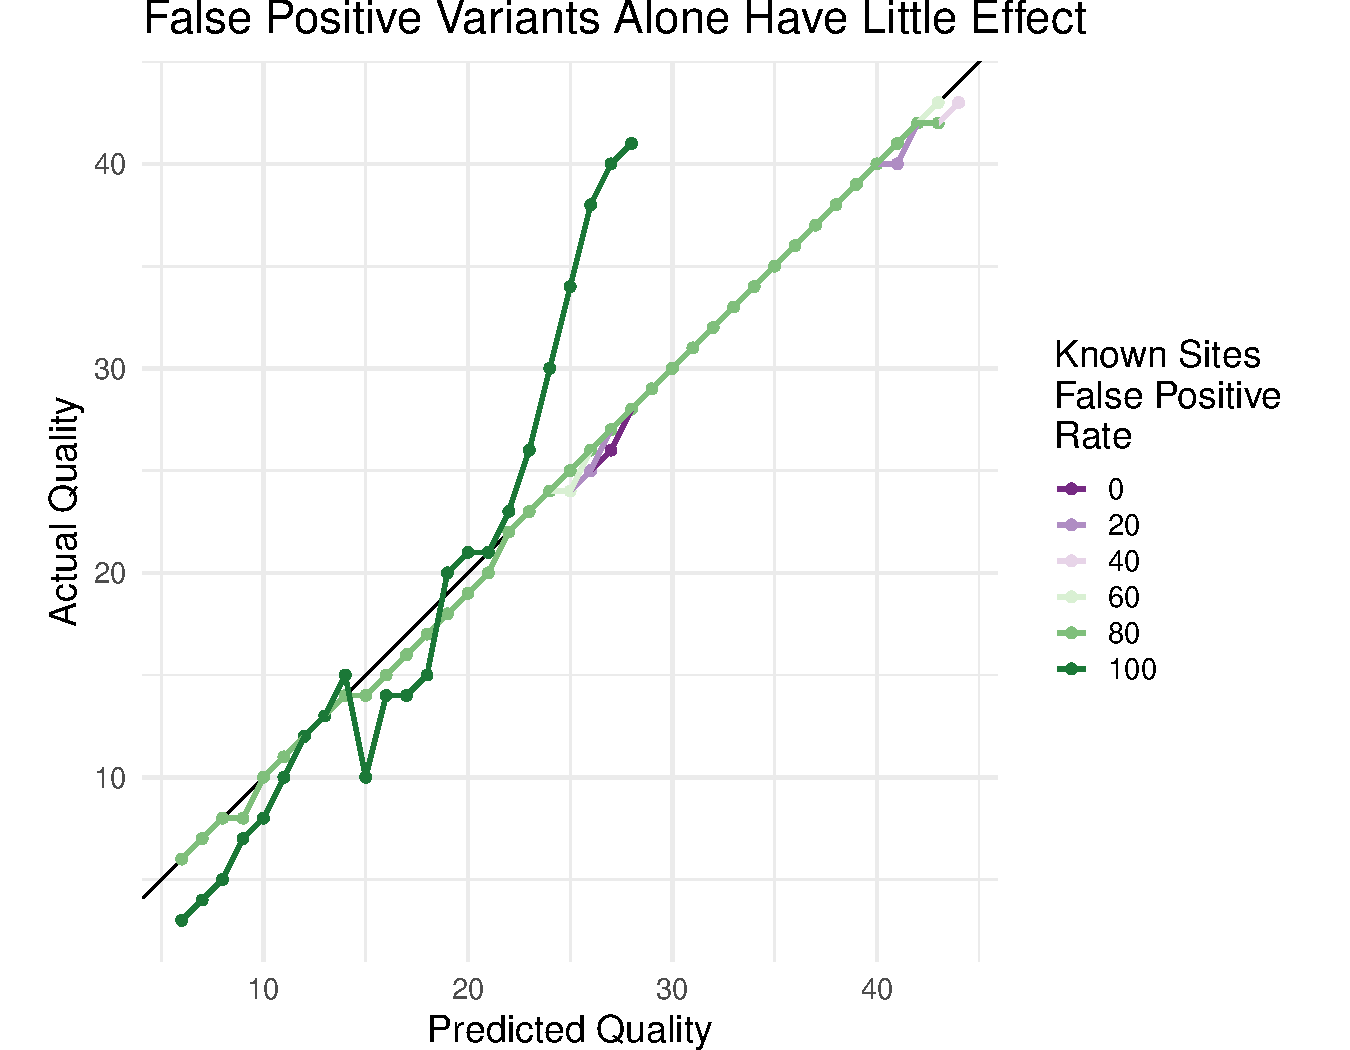
\includegraphics[width = .6\textwidth]{fpr.pdf}
	\titlecaption{False Positive Only Calibration}{Base quality score calibration for a range of false positives in the database of variable sites. The false negative rate for all datasets is zero. Increasing the false positive rate does not significantly impact the quality of the calibration. The poor calibration at a 100\% false negative rate is likely an artifact (see Section \ref{sec:kbbq_discussion}).}
	\label{figure:fpr}
\end{figure}

\begin{table}
\centering
\begin{tabular}{r l}
\toprule
False Positive Rate & RMSE \\
\midrule
0 & 0.60 \\
20 & 0.58 \\
40 & 0.53 \\
60 & 0.49 \\
80 & 0.49 \\
100 & 5.50 \\
\bottomrule
\end{tabular}
\titlecaption{False Positive Calibration Errors}{The root mean squared error of quality score for reads recalibrated using a database of variable sites with different false positive rates. The false negative rate for each dataset is 0\%.}
\label{table:fpr}
\end{table}

I also simulated different databases of variable sites with differing false negative rates and similarly used it to recalibrate my dataset. In these datasets, the false positive rate is 0\%. The plotted calibration and RMSE of the recalibrated data is shown in figure \ref{figure:fnr} and table \ref{table:fnr}. As the false negative rate increases, the degree of miscalibration also steadily increases.

\begin{figure}
	\centering
	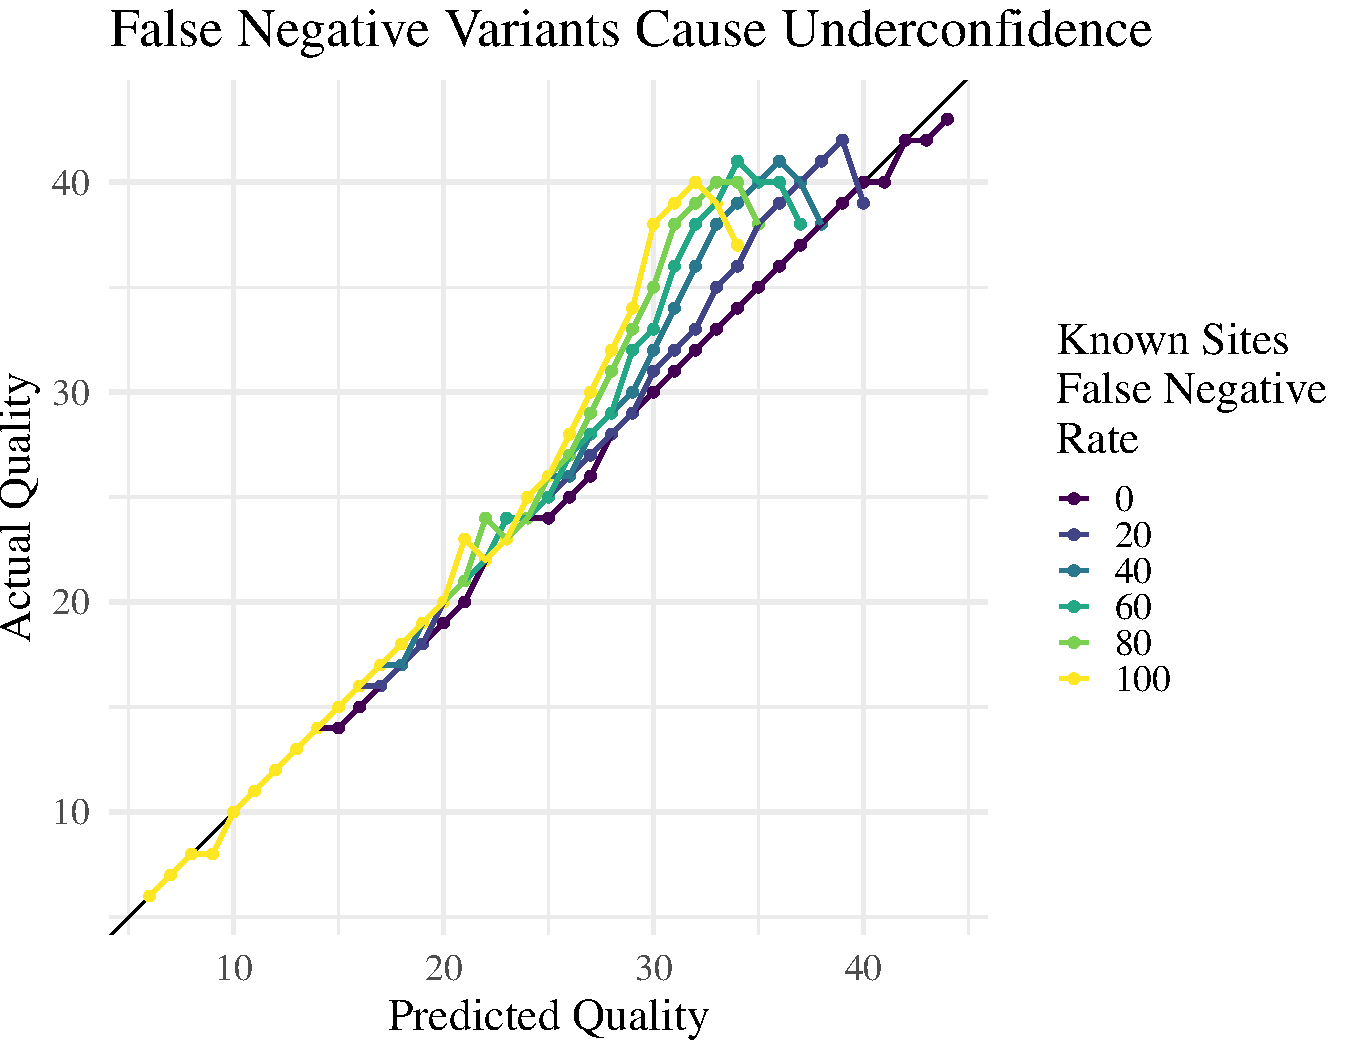
\includegraphics[width=.6\textwidth]{fnr.pdf}
	\titlecaption{False Negative Only Calibration}{Base quality score calibration for a range of false negatives in the database of variable sites. The false positive rate for all datasets is zero. Increasing the false negative rate significantly decreases the quality of the calibration, causing increasing  underconfidence in quality scores as the false negative rate rises.}
	\label{figure:fnr}
\end{figure}

\begin{table}
\centering
\begin{tabular}{r l}
\toprule
False Negative Rate & RMSE \\
\midrule
0 & 0.60 \\
20 & 1.32 \\
40 & 2.10 \\
60 & 2.57 \\
80 & 2.90 \\
100 & 3.20 \\
\bottomrule
\end{tabular}
\titlecaption{False Negative Calibration Errors}{Root mean squared error of quality score for reads recalibrated with a database of variable sites simulated with the given false negative rate. The false positive rate for each dataset is 0\%.}
\label{table:fnr}
\end{table}

To see if there were any interactive effects of false positive rate and false negative rate, I also simulated datasets with varying false positive and false negative rates. The RMSE of the calibrated scores is reported in Table \ref{table:fnrfpr} and summarized in Figure \ref{figure:fnrfpr}. These datasets were simulated separately from the above datasets, so there are slight differences in the calibration of the resulting reads.
As before, the number of false negatives significantly impacted calibration quality. In contrast to the false positive only dataset with a 0\% false negative rate, increasing the false positive rate also increased the amount of error in the calibration. Thus, false positives in the database of variable sites seem to enhance miscalibration caused by false negatives.

\begin{figure}
	\centering
	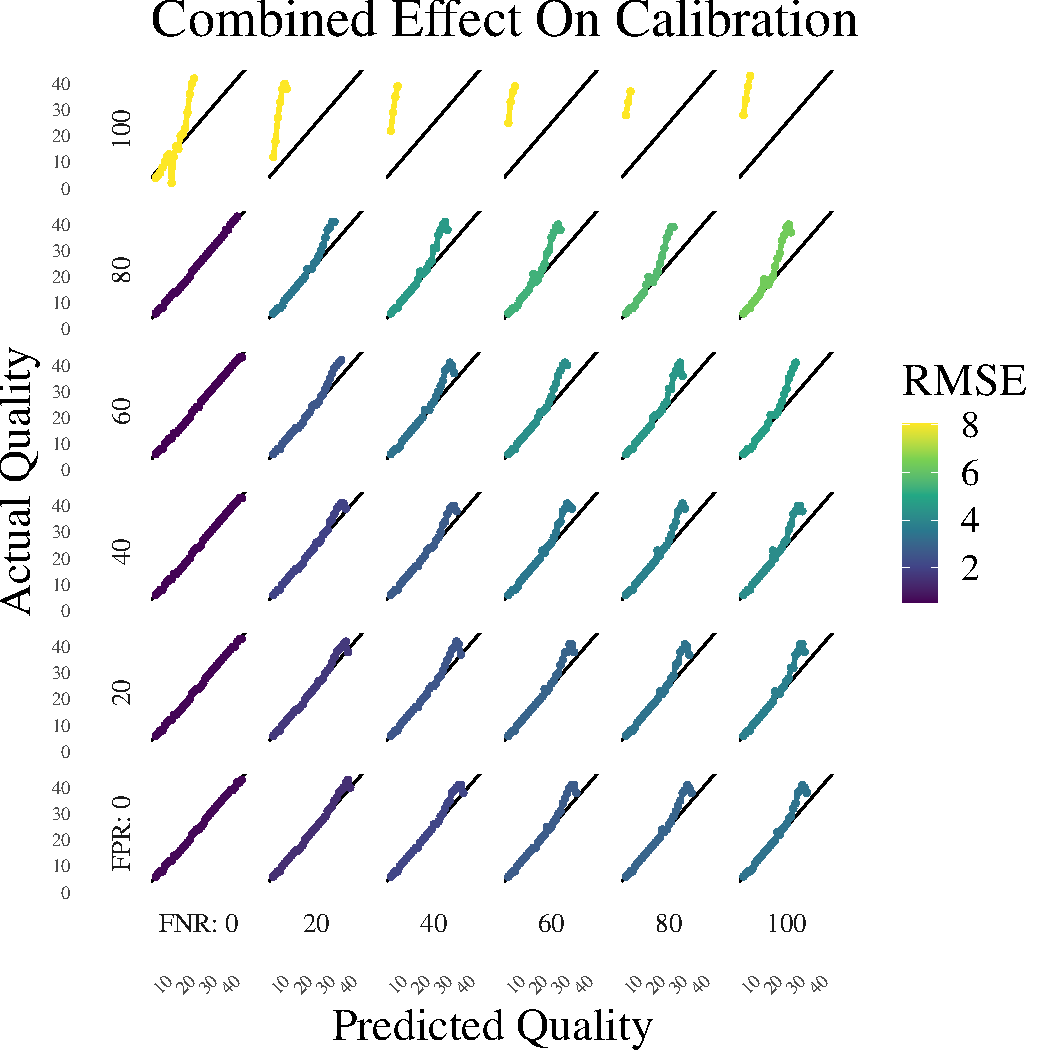
\includegraphics[width = \textwidth]{fnrfpr.pdf}
	\titlecaption{Combined Calibration}{Calibration of base quality scores of reads recalibrated using a database of variable sites with varying ranges of false negatives and false positives. The RMSE of the quality scores of the resulting calibration are used to color each line. Across the columns are each false negative rate, and each row represents a false positive rate. Except for at a false negative rate of 0, increasing either the false positive rate or the false negative rate increases the RMSE. See Table \ref{table:fnrfpr} for the RMSE values and the discussion in Section \ref{sec:kbbq_discussion} about false positive rates of 100\%}
	\label{figure:fnrfpr}
\end{figure}

\begin{figure}
	\centering
	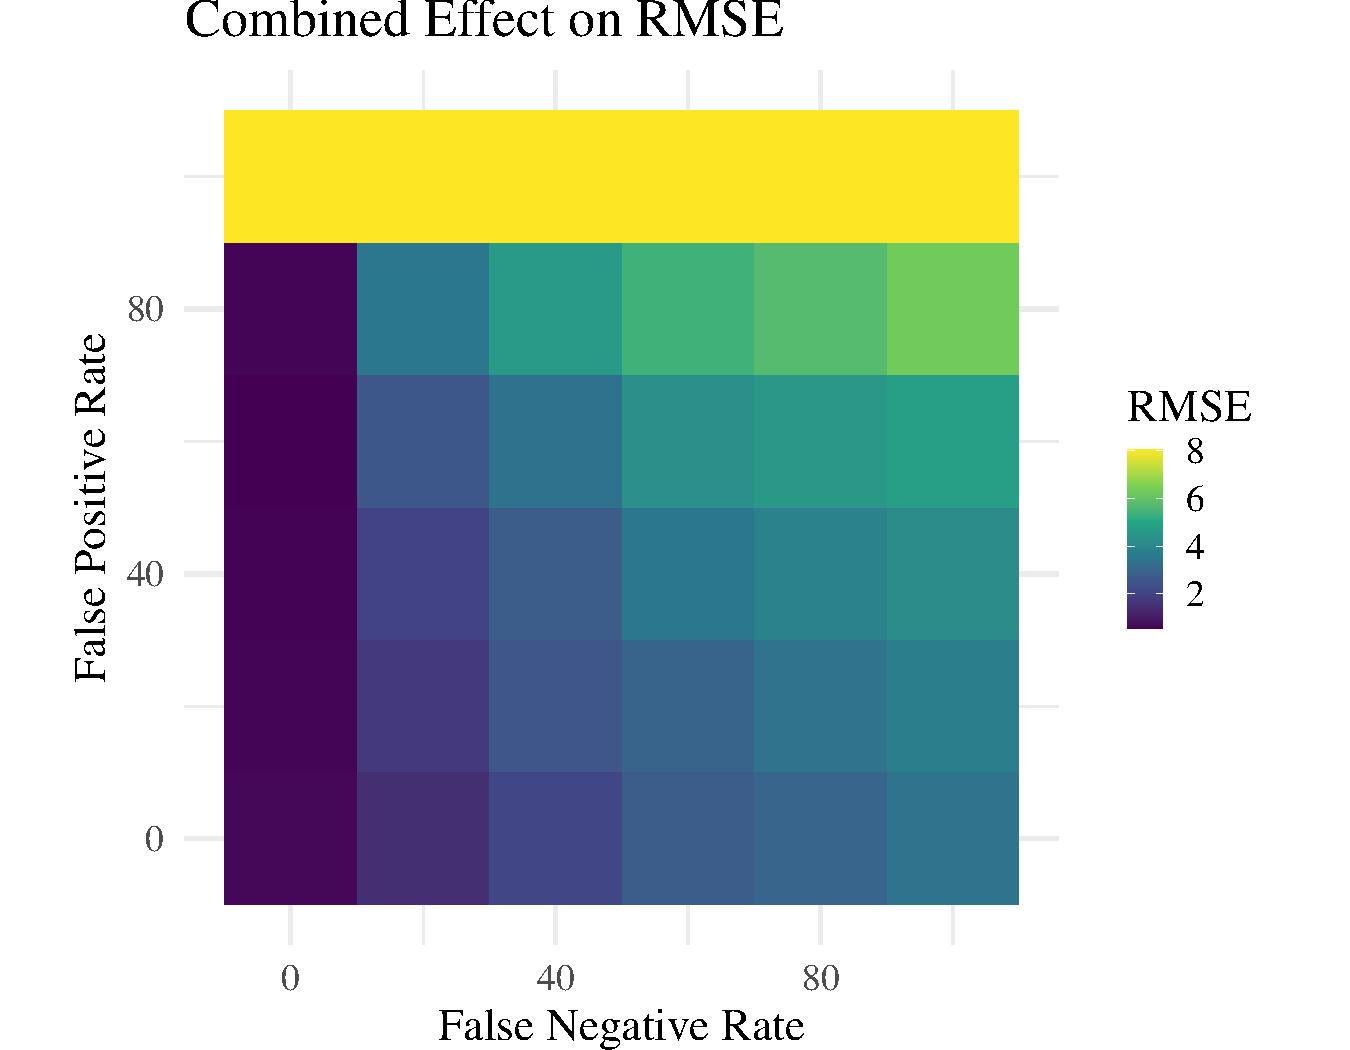
\includegraphics[width = .6\textwidth]{fnrfpr_heatmap.pdf}
	\titlecaption{Combined Calibration Heat Map}{Heat map of base quality calibration of varying ranges of false negatives and false positives. Databases of variable sites with differing false positive and false negative rates were constructed and the RMSE of the quality scores of the resulting calibration were calculated. Across the columns are each false negative rate, and each row represents a false positive rate. Except for at a false negative rate of 0, increasing either the false positive rate or the false negative rate increases the RMSE. See Table \ref{table:fnrfpr} for the RMSE values and the discussion in Section \ref{sec:kbbq_discussion} about false positive rates of 100\%}
	\label{figure:fnrfpr_heat}
\end{figure}

\begin{table}
\centering
\begin{tabularx}{.5\textwidth}{ l  X  X  X  X  X  X }
\toprule
\multirow{2}{*}{FPR} & \multicolumn{6}{c}{FNR} \\ \cmidrule(lr){2-7}
    & 0    &   20 &   40 &   60 &   80 &   100 \\
%&    &      &      &      &      &      & \\ %blank line
\midrule
0   & .641 & 1.45 & 2.08 & 2.73 & 2.99 & 3.38 \\
20  & .599 & 1.73 & 2.54 & 2.96 & 3.39 & 3.76 \\
40  & .555 & 2.02 & 2.71 & 3.50 & 3.84 & 4.16 \\
60  & .531 & 2.58 & 3.37 & 4.27 & 4.51 & 4.73 \\
80  & .593 & 3.52 & 4.62 & 5.38 & 5.73 & 6.32 \\
100 & 8.05 & 22.0 & 24.3 & 26.4 & 25.8 & 28.9 \\
\bottomrule
\end{tabularx}
\titlecaption{Combined Calibration Errors}{Root mean squared error of base quality score for data calibrated with databases of variable sites containing different levels of false positives and false negatives. The columns indicate false positive rates, the rows indicate false negative rates. The values in each cell are the RMSE of the quality scores for the reads recalibrated with the database of variable sites with false positive and false negative rate appropriate for its row and column. See Figure \ref{figure:fnrfpr_heat} for a graphical representation. The data in the 100\% false positive rows are likely artifacts; see section \ref{sec:kbbq_discussion} for more information.}
\label{table:fnrfpr}
\end{table}

Using GATK's recommended method of using high-confidence variants when a database of variable sites is unavailable produced poorly calibrated data with a RMSE of 1.66. This RMSE is similar to the RMSE of a simulated dataset with a false negative rate of approximately 20\%and a false positive rate between 0 and 20\%. However, the shape of this recalibrated data is also interesting; it seems that the major effect of recalibration was squeezing high quality scores toward the mean, as the highest recalibrated score in the dataset is 34 whereas using the truth set of variants yielded a highest recalibrated score of 44. This calibration and the calibration using the truth set, using KBBQ, and the raw read quality are plotted in Figure \ref{figure:comparison} and the RMSEs of each data set is listed in Table \ref{table:comparison}

\begin{figure}
\centering
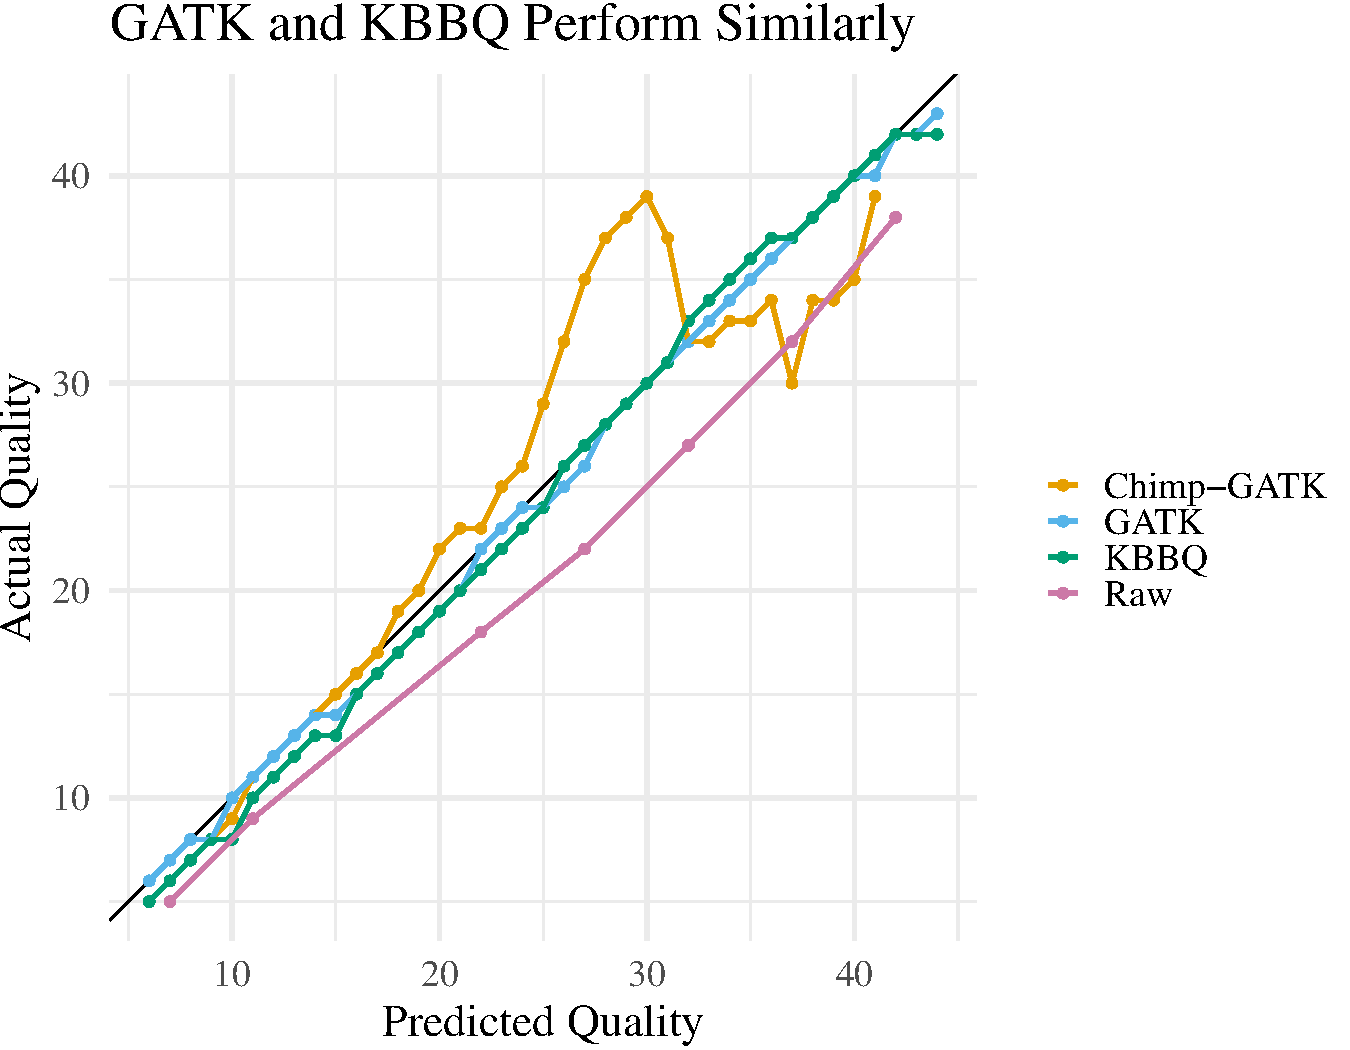
\includegraphics[width = .6\textwidth]{comparison.pdf}
\titlecaption{Comparison of Calibration Methods}{Chimp-GATK is the result of calibrating the reads using the model trained on the reads aligned to the chimp genome along with the variants called using that alignment. GATK is the result of using GATK's BaseRecalibrator with the truth set of variants. KBBQ is the result of using the KBBQ tool, which requires only reads and no reference or variant set. Raw is the calibration of the uncalibrated data.}
\label{figure:comparison}
\end{figure}

\begin{table}
\centering
\begin{tabular}{r l}
\toprule
Calibration Method & RMSE \\
\midrule
Chimp-GATK & 1.66 \\
GATK & 0.60 \\
KBBQ & 0.96 \\
Raw & 4.05 \\
\bottomrule
\end{tabular}
\titlecaption{Errors of Different Calibration Methods}{Root mean squared error of quality score for reads recalibrated using different methods. Chimp-GATK is the result of calibrating the reads using the model trained on the reads aligned to the chimp genome along with the variants called using that alignment. GATK is the result of using GATK's BaseRecalibrator with the truth set of variants. KBBQ is the result of using the KBBQ tool, which requires only reads and no reference or variant set. Raw is the calibration of the uncalibrated data.}
\label{table:comparison}
\end{table}

% \begin{outline}	
	% - do this for CH3 
	% \item Simulate downstream effect of FP and FN on variant quality; perhaps can do this with F-score - this should be done for CH3
	% \item Perhaps look at depth vs. variant quality to see if BQSR helps more in low-coverage scenarios - this should be done for CH3
	% \item Application
	% \begin{outline}
	% 	\item Describe Eucalyptus data
	% 	\item Describe structure in data that enables estimating the false positive and false negative rate
	% 	\item Recalibrate reads with \texttt{kbbq} instead of GATK BQSR and see how variant FPR and FNR change.
	% \end{outline}
% \end{outline}

\section{Discussion}
\label{sec:kbbq_discussion}
These results show that GATK BaseRecalibrator is particularly vulnerable to false negatives (Figure \ref{figure:fnr}) in the database of variable sites, but is robust to false positives if the false negative rate is near 0 (Figure \ref{figure:fpr}). At the same time, when the false negative rate is not near 0, false positives will start to impact the calibration quality (Figure \ref{figure:fnrfpr}). Thus, when this database is unavailable and construction is required, it may be better to be liberal in deciding which sites may be variable to reduce the false negative rate as much as possible. This is in contrast to the GATK recommendation to use only the most confident sites when a database is unavailable.

The only rate that shows significant deviation from a 0\% false positive rate in the false-positive-only data is the 100\% false positive rate. Though a 100\% false positive rate with a 0\% false negative rate implies every site should be considered variable and ignored, the model curiously still has a source of errors it uses to recalibrate. Upon further investigation, this effect is driven by reads with alignments that begin with an insertion, as these inserted bases are not ignored by BaseRecalibrator when the first position of the site that should be ignored is equal to the first aligned position in the read. Thus, this line is a technical artifact. So long as there are enough bases available to analyze, the false positive rate doesn't significantly affect the performace of BaseRecalibrator at a false negative rate of 0. The calibrations of other datasets with a false positive rate of 100\% would also be affected by this artifact; however, in a real dataset it's unlikely to ever achieve a false positive rate of 100\%, so this artifact is unlikely to significantly affect real data.

%new para
Ultimately, if the false negative and false positive rates of the database of variable sites is high, GATK's procedure for BQSR \textit{can} cause miscalibration of the data worse than using raw quality scores, though this can only happen with very large error rates. In this dataset, the raw data has a RMSE of about 4, which is similar to a simulated dataset with a false negative rate between 40-60\% and a false positive rate between 60-80\%. In a real situation it's unlikely that error rates like this will occur, so BQSR will not severely destroy the input data. However, at even modest false negative and false positive error rates BQSR can cause undesirable miscalibration that could feasibly impact variants called from the data. Interestingly, at all error rates the calibration of quality scores below 25 is almost always correct or 1-off the true value. It seems that errors in the database of variable sites have a larger effect on higher quality predictions than lower ones.

At the same time, the calibration model trained with the chimp-aligned data shows performance worse than a simulated dataset with a false negative rate of approximately 20\%. While the RMSE of 1.66 is not particularly high, the plotted calibration shows very poor performance at higher quality scores, and the maximum quality score the model assigned was 34 in contrast to other methods, which had a maximum assigned score of 44. Additionally, all quality scores assigned above 30 were more than one off the true quality score. And while all the simulated datasets caused underconfidence in the calibration, this calibration method caused overconfidence.

This suggests that an effect not captured in the simulated data was present in this data. Overconfidence indicates errors that should be counted by the model are instead missed and therefore there are more errors in actuality than the model predicts. Thus the set of variants used to skip errors is too aggressive and contains many false positives. So why is a similar effect not observed in the simulated data? This is likely because of how the simulated datasets were constructed; non-variable sites were selected independently and at random to be added to the set of purported variable sites. Thus a site containing an error and a site not containing an error are selected proportionally. In contrast, on a real dataset a variant calling algorithm would not make false positive errors independently; it is much more likely to classify a site as variable that has a sequencing error than to classify a site as variable that has no errors. That is: in this simulation, $P(\operatorname{classified\:positive} | \operatorname{actual\:negative})$ is independent of $P(\operatorname{sequencing\:error})$, but on an empirical dataset $P(\operatorname{classified\:positive} | \operatorname{actual\:negative})$ is likely not. Thus in reality false positives probably cause overconfidence in a similar manner that false negatives cause underconfidence. This overconfidence is observed in this calibration method.

As the chimp-aligned calibration shows, GATK BQSR struggles on real data from non-model organisms. False negatives are likely to be numerous in almost all but the most well-studied samples \parencite{bobo_false_2016}, and false positives are similarly likely when using poor quality, draft reference genomes that cause alignment errors. This means in most datasets, while its performance may be acceptable if the false negative and false positive rate are sufficiently low, GATK BaseRecalibrator is not the best recalibration method. This is shown in Figure \ref{figure:comparison}, which shows \texttt{kbbq} performing nearly as well as GATK BQSR with perfect knowledge of variable sites. However, \texttt{kbbq} doesn't use any reference or any variant site information to do recalibration. \texttt{kbbq} also performs much better than GATK's recommended procedure when a database of variable sites is not available, as shown in the Chimp-GATK calibration.

\section{Conclusion}

Base quality score recalibration is an important procedure to ensure base quality scores are accurate before variant calling. However, the most popular method for doing BQSR is not easy to do if the sequenced organism is a non-model organism. I simulated sets of variable sites with varying false positive and false negative rates to use with BQSR. While it seems the simulated false positives are somewhat different from those that appear in real datasets, it is clear that false negatives severely reduce the quality of the calibration using GATK's method. I developed the software tool \texttt{kbbq} to recalibrate base quality scores without a reference or database of variable sites to overcome these deficiencies. Since it doesn't use a database of variable sites or a reference, the quality of these resources is immaterial to the quality of the resulting calibration. Finally, I emulated GATK's procedure for calibration when a database of variable sites is unavailable by aligning benchmark data to the chimp genome and calling variants to use as the database of variable sites. This method produces a calibration much worse than \texttt{kbbq}. Thus, when a database of variable sites or reference is unavailable or of poor quality, \texttt{kbbq} is an effective method for base quality score recalibration.

\printbibliography[segment=\therefsegment]{}

	% \item Future work: see how big the difference is in variant calls using binned quality scores, miscalibrated reads, and well calibrated reads.
